
\documentclass{article}
\usepackage{graphicx} % Required for inserting images
\usepackage{amsfonts}
\usepackage{hyperref}
\usepackage{amsmath} 
\usepackage{booktabs}
\usepackage{float}

\title{24.08.20 MuSig2, SpeedyMuSig and Shuffle Arguement}
\author{Xun Zhang \quad \quad Wuyun Siqin \quad \quad Bingsheng Zhang \\ 
Zhejiang University, CHN \\
22221024@zju.edu.cn \quad 3210101763@zju.edu.cn \quad bingsheng@zju.edu.cn}

\date{August 20 2024}
\begin{document}

\maketitle

\section{MuSig2 Benchmark}

We implemented the MuSig2 scheme, this SNARK-based multi-signature scheme prove the following statements:
\begin{enumerate}
    \item $a_i = \textrm{H}_{agg1}(L || X_i)$ for all $X_i$, where $L = (X_1, X_2, ... , X_n)$
    \item $X = a_1*X_1 + a_2*X_2 +...+ a_n*X_n$
    \item $R' = R_1' + R_2' +...+ R_n'$
    \item $R'' = R_1'' + R_2'' +...+ R_n''$
    \item $b = \textrm{H}_{agg2}(X||R'||R''||m)$
    \item $R_i = R_i'+bR_i''$ for all $(R_i',R_i'')$
    \item $R = R_1 + R_2 +...+ R_n$
    \item $s = s_1 + s_2 + ... + s_n$
    \item $s*G =? R+\textrm{H}_{sig}(X, R, msg)*X$
\end{enumerate} 

Note that this is the whole workflow of MuSig2. The benchmark results are as follows:

\begin{table}[H]
    \centering
    \begin{tabular}{c|c} \hline
        Settings & Proof Time \\ \hline
        k=14, n=6 & 1.3837s \\ \hline
        k=15, n=15 & 2.5438s \\ \hline
        k=16, n=30 & 4.8002s \\ \hline
        k=17, n=60 & 8.6175s  \\ \hline
        k=18, n=120 & 17.392s \\ \hline
    \end{tabular}
    \caption{Benchmark results for MuSig2}
    \label{tab:version1_agg}
\end{table}

\section{SpeedyMuSig Benchmark}

We implemented the SpeedyMuSig scheme, this SNARK-based multi-signature scheme prove the following statements:

\begin{enumerate}
    \item $X = \sum_{i=1}^{n} X_i$
    \item $R' = R_1' + R_2' +...+ R_n'$
    \item $R'' = R_1'' + R_2'' +...+ R_n''$
    \item $b = \textrm{H}_{agg2}(X||R'||R''||m)$
    \item $R_i = R_i'+bR_i''$ for all $(R_i',R_i'')$
    \item $R = R_1 + R_2 +...+ R_n$
    \item $s = s_1 + s_2 + ... + s_n$
    \item $s*G =? R+\textrm{H}_{sig}(X, R, msg)*X$
\end{enumerate} 

We assume that the aggregator has verified all the proof-of-possession signatures from signers. Thus this part of computation is not included in circuit.



\begin{table}[H]
    \centering
    \begin{tabular}{c|c} \hline
        Settings & Proof Time \\ \hline
        k=13, n=6 & 0.7817s \\ \hline
        k=14, n=15 & 1.3665s \\ \hline
        k=15, n=30 & 2.4466s \\ \hline
        k=16, n=60 & 4.5086s  \\ \hline
        k=17, n=120 & 8.3763s \\ \hline
    \end{tabular}
    \caption{Benchmark results for SpeedyMusig}
    \label{tab:version1_agg}
\end{table}

\section{Comparison}

We offer a quick comparison of three Schnorr multi-signature schemes:


\begin{table}[H]
    \centering
    \begin{tabular}{|c|c|c|c|} \hline
        & MuSig & MuSig2 & SpeedyMuSig \\ \hline
       Signature Scheme& Schnorr &Schnorr &Schnorr \\ \hline
       Assumption & DL & AOMDL & AOMDL \\ \hline
       Offline Round & 1 &1 & 1 \\ \hline
       Online Round & 2 & 1 & 1 \\ \hline
       PK Aggregation & Heavy & Heavy & Simple \\ \hline
    \end{tabular}
    \caption{MuSig Comparison}
    \label{tab:version1_agg}
\end{table}


Due to the simple aggregation method of PKs, the SpeedyMuSig scheme is about 2x faster than other schemes in Halo2 proving.


\section{Mithril Discussion}

We offer a discussion about Mithril, about its public keys aggregation, security consideration and potential SNARK-version realization.

\subsection{Public Keys Aggregation}

The aggregation technology of Mithril is similar to MuSig and MuSig2. In the original paper:

\begin{itemize}
    \item $\textrm{MSP.BKey}(\mathbf{mvk, e_\sigma})$:Takes a vector $\mathbf{mvk}$ of (previously checked) verification keys and weighting seed $e_\sigma$, and returns an intermediate aggregate public key $ivk=\prod mvk_i^{e_i} $, where $e_i \leftarrow \textrm{H}(i,e_\sigma)$.
    \item $\textrm{MSP.BSig}(\mathbf{\sigma})$:Takes as input a vector of signatures $\mathbf{\sigma}$ and returns $(\mu, e_\sigma)$ where $\mu \leftarrow \prod \sigma_i^{e_i}$, where $e_i \leftarrow \textrm{H}(i,e_\sigma)$ and $e_\sigma \leftarrow \textrm{H}(\sigma)$.

\end{itemize}

The paper also said that:

\textit{The $\mathrm{MSP.BKey}$ and $\mathrm{MSP.BSig}$ aggregation functions enforce more stringent checking than that of standard multisignatures by utilizing the short random exponent batching of Bellare et al. The difference from standard multisignature aggregation, is that the randomized check will fail with overwhelming probability if any of the individual signatures is invalid, whereas the simpler aggregation allows for erroneous individual signatures if the aggregate is correct.}


\subsection{Mithril and SpeedyMuSig}

In SpeedyMuSig scheme, there is a same proof-of-possession process, just as same as Mithril. But SpeedyMuSig avoid the complex public keys aggregation method, replace it by a simple product of public keys.

The SpeedyMuSig paper claimed that they prove the EUF-CMA security of SpeedyMuSig in the programmable random oracle model under the one-more discrete logarithm assumption and the Schnorr knowledge of exponent assumption. 

\subsection{SNARK-based Mithril}

we give a quick review of what we have done to SNARK-based Mithril:

\begin{enumerate}
    \item $ivk = \prod mvk_i$
    \item $\mu \leftarrow \prod_{i=1}^d \sigma_i$
    \item $e(g1, \sigma) = e(ivk, \textrm{H}(m))$
    \item $\textrm{root} = \textrm{H}(mvk,...)$, and all $mvk_i \in (mvk, ...)$
\end{enumerate}

Note that the original Mithril paper verify the BLS signature like: $e(\sigma, g2) = e(\textrm{H}_{\mathbb{G}_1}(''M''||msg), ivk)$. Since it is a preliminary implementation, we can modify it later.

Our preliminary plan is to implement the following form of SNARK-based Mithril.

\begin{enumerate}
    \item $ivk=\prod mvk_i^{e_i} $, where $e_i \leftarrow \textrm{H}(i,e_\sigma)$.
    \item $\mu \leftarrow \prod \sigma_i^{e_i}$, where $e_i \leftarrow \textrm{H}(i,e_\sigma)$ and $e_\sigma \leftarrow \textrm{H}(\mathbb{\sigma})$.
    \item $e(g1, \mu) = e(ivk, \textrm{H}(m))$
    \item $\textrm{root} = \textrm{H}((mvk,stake),...)$, and all $(mvk_i, stake_i) \in ((mvk,stake),...)$
\end{enumerate}

This could be challenging. And we are still searching for better solution of zero-knowledge bridge for Cardano.










\section{Shuffle Arguement Discussion}

\subsection[BG12]{\texorpdfstring{BG12\footnote{Bayer, S., Groth, J.:Efficient Zero-Knowledge Argument for Correctness of a Shuffle. In:EUROCRYPT 2012.}}}\label{bg121}


\textbf{Common Reference String:} $\mathsf{pk}, \mathsf{ck}$.

\textbf{Statement:} $\mathcal{C}, \mathcal{C'} \in \mathbb{H}^N$ with $N = mn$.


\textbf{Witness:} The prover possesses a permutation $\pi \in \Sigma_N$ and randomness $\rho \in \mathbb{Z}_q^N$ such that $C' = \mathcal{E}_{\mathsf{pk}}(1; \rho) C_\pi$.

\textbf{Proof Phases:} 
\begin{enumerate}
\def\labelenumi{\arabic{enumi}.}
\item 
P: Commit to $\mathbf{a} = \{\pi(i)\}_{i=1}^N$.
\item
V: Pick $x \leftarrow \mathbb{Z}_q^*$ as the challenge.
\item 
P: Commit to $\mathbf{b} = \{x^{\pi(i)}\}_{i=1}^N$ .
\item 
V: Pick $y, z \leftarrow \mathbb{Z}_q^*$ as the challenge.
\item 
P: Compute and commit to $\mathbf{d} = y\mathbf{a} +\mathbf{b}$ , $\mathbf{-z} = (-z,-z,...,-z,\mathbf{0})$

Compute $\rho = -\mathbf{\rho} \cdot \mathbf{b}$ and set $\mathbf{x} = (x, x^2, \ldots, x^N)^T$.

\end{enumerate}

\textbf{Verification:} The verifier checks the commits to a and b ,$\mathbf{c}_a, \mathbf{c}_b \in \mathbb{G}^m$ and computes $\mathbf{c}_{-z}$ and $\mathbf{c}_d$ along with $\mathbf{C}^\mathbf{x}$ and $\prod_{i=1}^N (y i + x^i - z)$.

Engage in a product argument for the openings of $\mathbf{d} - \mathbf{z}$ , and verify the equality
\[
\prod_{i=1}^N (d_i - z) = \prod_{i=1}^N (y i + x^i - z).
\]
Engage in a multi-exponentiation argument of $\mathbf{b}$ and $\rho$ such that:
\[
\mathbf{C}^\mathbf{x} = \mathcal{E}_{\mathsf{pk}}(1; \rho) \mathbf{C'}^\mathbf{b}
\]

The verifier accepts if the product and multi-exponentiation arguments are both valid.

\subsection{A Naive Approach}

For cases where it is unnecessary to hide the ciphertext and the permutation \(\pi\), a simplified method can be employed: treat the vector \( C' \) as a permutation of the vector \( C \). Introduce a challenge value \( z \) and then compute the product of each element of \( C \) and \( C' \) after subtracting \( z \). If the results of the two products are equal, it indicates that \( C' \) is indeed a permutation of \( C \).

The mathematical description is as follows:

\begin{enumerate}
    \item Compute \( \prod_{i=1}^{n} (c_i - z) \).
    \item Compute \( \prod_{i=1}^{n} (c'_i - z) \).
\end{enumerate}

If the following equality holds:

\[
\prod_{i=1}^{n} (c_i - z) = \prod_{i=1}^{n} (c'_i - z)
\]

then \( C' \) is a permutation of \( C \). There's no need the possession of the permutation $\pi$.

This approach essentially constructs polynomials with respect to \( z \) from the two vectors. According to Schwartz-Zippel lemma, the prover has negligible chance over the choice of z of making a convincing argument unless indeed there is a permutation $\pi$.

% \subsection{Cost discussion}





\section{Halo2-lib Benchmark}


\subsection{Bug Discussion}

\begin{figure}[H]
    \centering
    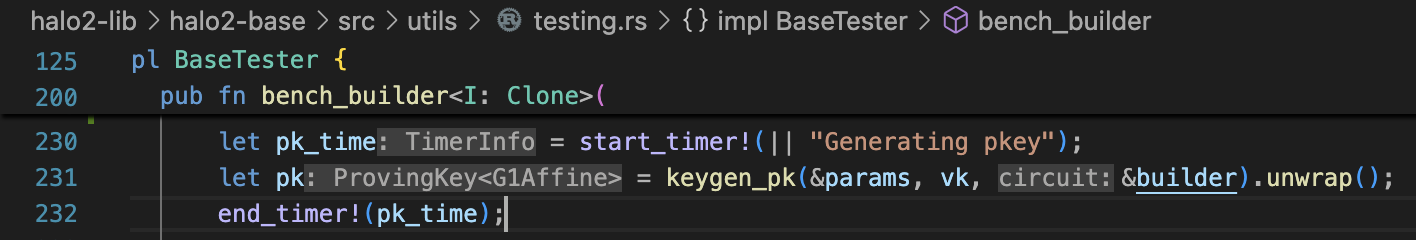
\includegraphics[width=1\linewidth]{bug1.png}
    \caption{Use of TimerInfo}
    \label{fig:enter-label}
\end{figure}

The issue in the code snippet is related to the end\_timer! macro. The problem is that end\_timer! does not actually stop the timer immediately when it is called. Instead, it stops the timer only when the elapsed function is subsequently invoked. This causes a cumulative effect on the recorded time, leading to an inaccurate total duration. Specifically, the time keeps accumulating until elapsed is called, which results in the final timing measurement including time that should not be accounted for.

\begin{figure}[H]
    \centering
    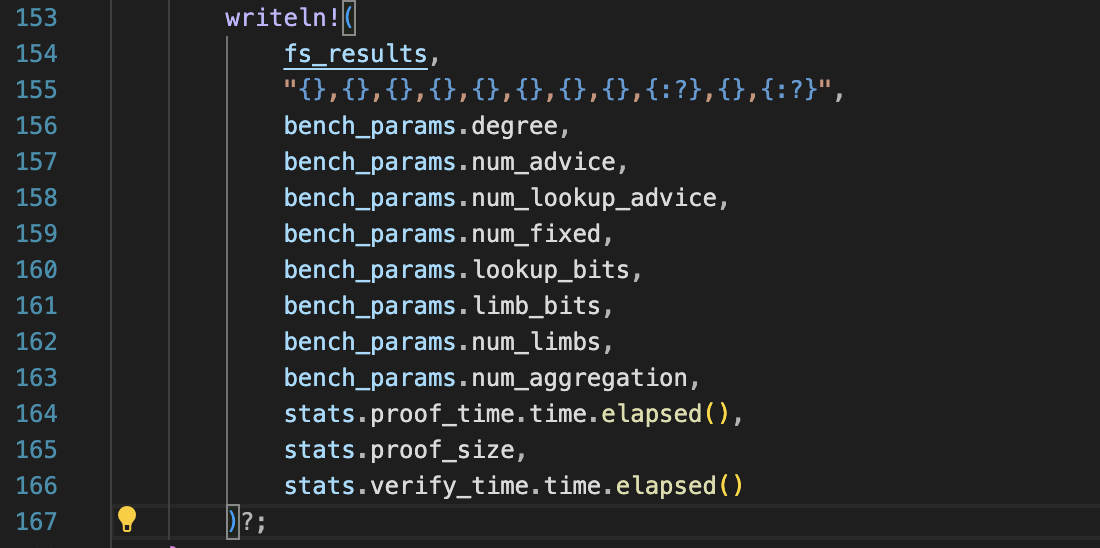
\includegraphics[width=1\linewidth]{bug2.png}
    \caption{When the Timer stop}
    \label{fig:enter-label}
\end{figure}

\subsection{New Test Results}

\begin{tabular}{c|c|c|c|c|c}
\hline
 degree &  num\_aggregation &  num\_origin &     proof\_time &  proof\_size &  verify\_time \\
\hline
     17 &              256 &         512 &  65.107423254s &       41632 &  22.065098ms \\
     17 &              512 &        1024 & 111.976211587s &       76448 &  34.824188ms \\
     17 &             1024 &        2048 & 223.437017328s &      150912 &   67.46092ms \\
     17 &             2048 &        4096 & 470.005966428s &      310336 & 124.343528ms \\
 \hline
     19 &              256 &         512 &  61.625703969s &       10688 &  12.830639ms \\
     19 &              512 &        1024 & 104.553267256s &       19104 &  14.696026ms \\
     19 &             1024 &        2048 & 204.119754992s &       37664 &  21.397588ms \\
     19 &             2048 &        4096 & 439.596726985s &       77312 &  41.115937ms \\
 \hline
     21 &              256 &         512 &  81.647671708s &        3424 &  12.611693ms \\
     21 &              512 &        1024 & 120.595740985s &        5376 &  19.456223ms \\
     21 &             1024 &        2048 & 214.113378674s &        9984 &  19.698181ms \\
     21 &             2048 &        4096 & 440.551034029s &       19904 &  19.534606ms \\
\bottomrule
\end{tabular}


\end{document}


